\chapter{Infraestructura}\label{infraestructura}

En este capítulo se presentan las tecnologías que se han usado para el desarrollo de este Trabajo de Fin de Máster, el entorno donde se realizan las pruebas, las librerías utilizadas, los algoritmos y el lenguaje de programación.\\

Los entornos de pruebas elegidos son actualmente el referente del software libre de la robótica a nivel mundial. Para este trabajo se ha elegido este conjunto por la buena integración que tienen entre sí y la accesibilidad para que otros elementos puedan integrarse en ellos

%%%%%%%%%%%%%%%%%%%%%%%%%%%%%%%%%%%%%%%%%%%%%%%%%%%%%%%%%%%%%%%%%%%%%%%%%%%%%%%%%%%%%%%%%%%%%%%%%%%%%%%%%%%%%%%%
\section{Lenguaje Python}
Python\footnote{\url{https://www.python.org/download/releases/2.7/}} es un lenguaje de programación interpretado cuya filosofı́a se basa en una sintaxis que favorezca un código legible. Es de tipado dinámico, multiplataforma y soporta orientación a objetos, programación imperativa y, en menor medida, programación funcional. Ofrece versatilidad y alta compatibilidad con el resto de componentes de la infraestructura.\\

Python se ha adoptado como un lenguaje estándar para el desarrollo de algoritmos de inteligencia artificial. Gracias a la sintaxis clara, permite crear prototipos y proyectos de una manera ágil y relativamente sencilla lo que aumenta el interés por su uso. Este asentamiento de Python favorece la creación de librerías que ayudan a la creación de elementos más grandes, evitando un desarrollo inicial en cada proyecto.\\

Este Trabajo de Fin de Máster utiliza Python en su versión $2.7$ (debido a las limitaciones del resto de componentes) para el desarrollo de todo el código del algoritmo de aprendizaje por refuerzo.

%%%%%%%%%%%%%%%%%%%%%%%%%%%%%%%%%%%%%%%%%%%%%%%%%%%%%%%%%%%%%%%%%%%%%%%%%%%%%%%%%%%%%%%%%%%%%%%%%%%%%%%%%%%%%%%%
\section{Biblioteca Numpy}\label{numpy}

Estándar asentado como librería de procesamiento de datos, es una extensión del lenguaje Python para operaciones con vectores y matrices. Numpy\footnote{\url{https://numpy.org/}}, en su versión $1.16.6$ se utiliza en el proyecto para facilitar los cálculos en la etapa de procesamiento de la imagen de entrada.\\

Numpy permite trabajar con estructuras matriciales N-dimensionales con relativa facilidad si se compara con las herramientas nativas de Python. Cuenta con un gran repertorio de métodos para gestionar los datos como: sistema de indexado y búsqueda, formateo de los datos, manipulación de la forma del dato, etc, lo que simplifica las operaciones con matrices o imágenes en este caso.

%%%%%%%%%%%%%%%%%%%%%%%%%%%%%%%%%%%%%%%%%%%%%%%%%%%%%%%%%%%%%%%%%%%%%%%%%%%%%%%%%%%%%%%%%%%%%%%%%%%%%%%%%%%%%%%%
\section{Biblioteca OpenCV}\label{opencv}

Para el procesamiento de las imágenes que toma el robot se utiliza la librería estándar en aplicaciones con visión artificial OpenCV\footnote{\url{https://opencv.org/}} (\textit{Open Computer Vision}) en su versión $4.2.0$. Fue creada inicialmente por Intel y liberada bajo software libre con licencia BSD. Es una librería para aplicaciones de visión artificial de propósito general que incluye muchísimas funciones de procesamiento de imágenes de todo tipo desde erosión, dilatación, convolución, flujo óptico, seguimiento, etc. Es multiplataforma y disponible en los lenguajes C++, Python y Java.\\

OpenCV hace hincapié en la baja latencia en su procesamiento para conseguir tiempos muy bajos y asegurar el tiempo real en los algoritmos que tiene incluidos por lo que es perfecta para usarse en software robótico.\\

Esta librería es usada en el código para el procesamiento de la imagen de entrada que captura la cámara incorporada en el robot.

%%%%%%%%%%%%%%%%%%%%%%%%%%%%%%%%%%%%%%%%%%%%%%%%%%%%%%%%%%%%%%%%%%%%%%%%%%%%%%%%%%%%%%%%%%%%%%%%%%%%%%%%%%%%%%%%
\section{Entorno robótico ROS}

Como librería en comunicación entre el robot (simulado) y el entorno donde se llevan a cabo el entrenamiento con aprendizaje por refuerzo se elige el \textit{sistema operativo robótico} (\textit{Robot Operating System}, \textit{ROS}\footnote{\url{https://www.ros.org/}} en adelante), en su versión \textit{Melodic Morenia}, programado en C++ y Python y que está mantenido por la Fundación de Robótica de Código Abierto (\textit{Open Source Robotics Foundation}, OSRF). ROS es un entorno para el desarrollo de software para robots que adquiere la funcionalidad de un sistema operativo dado que contiene elementos que así lo caracterizan como son: abstracción a nivel de hardware, control de dispositivos de bajo nivel, implementación de funcionalidad de uso común, paso de mensajes entre procesos y mantenimiento de los paquetes adicionales que pueden integrarse en él.\\

ROS gestiona los robots como \textit{nodos} que permiten ejecutar programas independientes en cada uno de ellos separando la lógica entre \textit{publicador} y \textit{suscriptor}. El \textit{publicador} (el robot) emite eventos que ROS denomina \textit{topics} a los cuales el programa se conecta como \textit{suscriptor}. Para este proyecto el sensor utilizado en el vehículo es una cámara simple adherida en la parte delantera de un robot modelado como un Fórmula 1 y que recogerá la información frontal mientras avanza. El suscriptor se conecta a uno de los \textit{topics} emitido por ROS para la cámara y recoger así la información sensorial y a otro \textit{topic} para la gestión de los motores poder ordenarle movimiento al robot.\\

El puente que se emplea entre la cámara en el vehículo y el programa es un paquete denominado \texttt{cv\_bridge} que \textit{traduce} la información recogida por la cámara a valores numéricos interpretables por el lenguaje de programación y compatible con las librerías de Numpy y OpenCV.\\

%%%%%%%%%%%%%%%%%%%%%%%%%%%%%%%%%%%%%%%%%%%%%%%%%%%%%%%%%%%%%%%%%%%%%%%%%%%%%%%%%%%%%%%%%%%%%%%%%%%%%%%%%%%%%%%%
\section{Simulador robótico Gazebo}

El entorno de pruebas en el cual se refleja el comportamiento del robot es el simulador robótico de código libre \textbf{Gazebo}\footnote{\url{http://gazebosim.org}} en su versión 9, mantenido también por la OSRF. Las principales características de este simulador son:\\

\begin{itemize}
    \item Es en 3D.
    \item Permite simular multitud de sensores como cámaras, láser, etc.
    \item Muy buena integración con ROS ofreciendo interfaces para los robots simulados.
    \item Es multirobot.
    \item Incluye un motor de físicas realistas\footnote{\url{http://gazebosim.org/blog/four_physics}} como: Bullet\footnote{\url{https://pybullet.org/wordpress/}}, \textit{Open Dynamics Engine (ODE)\footnote{\url{https://www.ode.org/}}}, \textit{Dynamic Animation and Robotics Toolkit} (DART) \footnote{\url{https://dartsim.github.io/}}, etc.
    \item Soporta muchísimos modelos diferentes de robot y permite modelarse utilizando URDF\footnote{\url{http://wiki.ros.org/urdf}}.\\
\end{itemize}

Por todas las características mostradas, es uno de los simuladores más usados en la comunidad investigadora internacional en robótica.\\

A través de los lanzadores de ROS (\texttt{roslaunch}) se configura el entorno donde se lanza la simulación y el mundo que contiene el robot así como los sensores y actuadores. En la figura \ref{fig:gazebo-nurburgring} puede verse un ejemplo de un \textit{mundo} de Gazebo empleado en este Trabajo Fin de Máster.

\begin{figure}[!ht]
    \centering 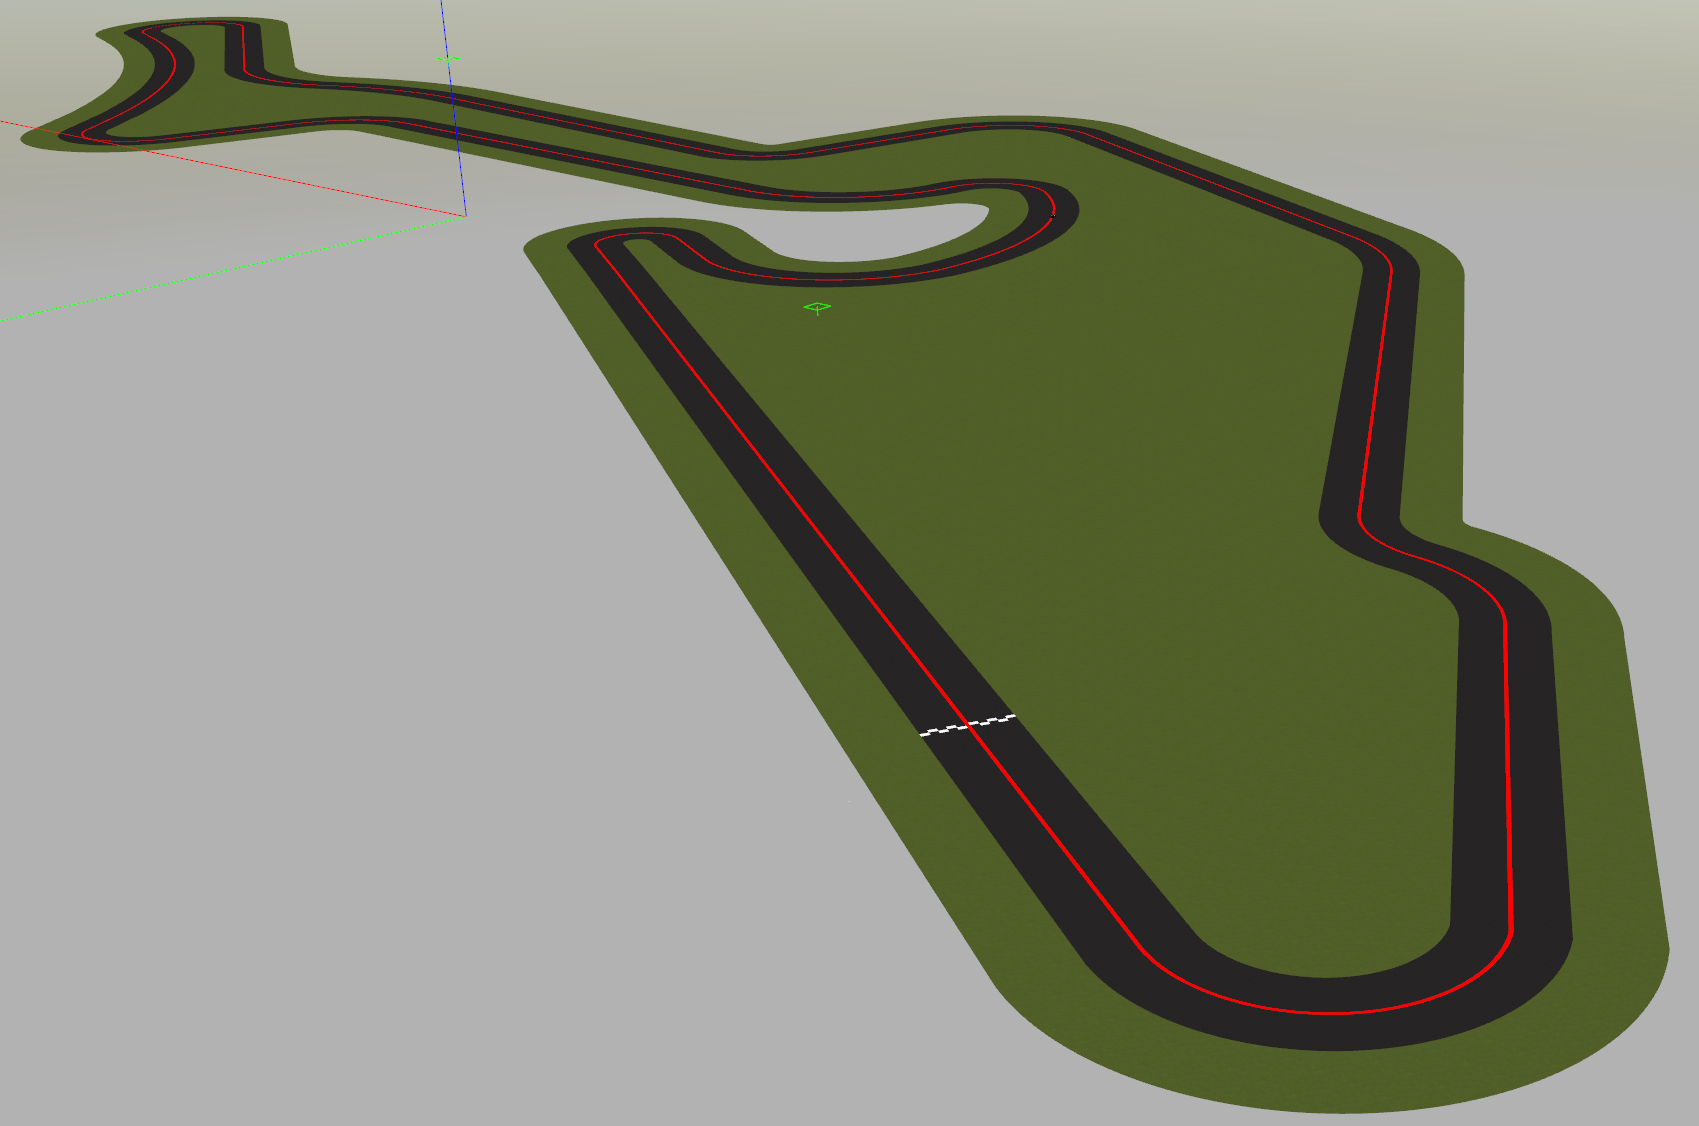
\includegraphics[width=0.5\columnwidth]{./figures/chapter_3/nurburgring.png}
    \caption{Réplica del circuito de Nürburgring en el simulador Gazebo.\label{fig:gazebo-nurburgring}}
\end{figure}


%%%%%%%%%%%%%%%%%%%%%%%%%%%%%%%%%%%%%%%%%%%%%%%%%%%%%%%%%%%%%%%%%%%%%%%%%%%%%%%%%%%%%%%%%%%%%%%%%%%%%%%%%%%%%%%%
\section{OpenAI Gym}

OpenAI Gym\footnote{\url{https://gym.openai.com/}} es una plataforma perteneciente a la empresa OpenAI que permite construir \textit{entornos} de investigación para probar diferentes algoritmos de aprendizaje por refuerzo. Está escrito en lenguaje Python y ofrece una capa de abstracción que permite al usuario elaborar espacios donde construir su código utilizando el mismo repertorio de funciones para cada uno de los entornos convirtiéndose en la plataforma de referencia en el aprendizaje por refuerzo.\\

Gym es popular por tener en su repertorio entornos de videojuegos procedentes (en su mayoría) de la consola Atari (figura \ref{fig:openai-gym}). A través de los distintos algoritmos de aprendizaje por refuerzo se demuestra que en cada entorno (o videojuego) funciona mejor un algoritmo en concreto para solucionar o completar el juego. Con los escenarios preparados, el usuario únicamente tiene que encargarse de programar la lógica del agente.\\

En la figura \ref{fig:openai-gym} se muestran algunos de los entornos de los que dispone OpenAI Gym para la ejecución de diferentes algoritmos de aprendizaje por refuerzo y por refuerzo profundo como: el juego de Breakout de la consola Atari, el problema del Cartpole, el ejemplo de un agente que aprende a caminar en el entorno de Bipedal Walker, etc.

\begin{figure}[!ht]
    \centering 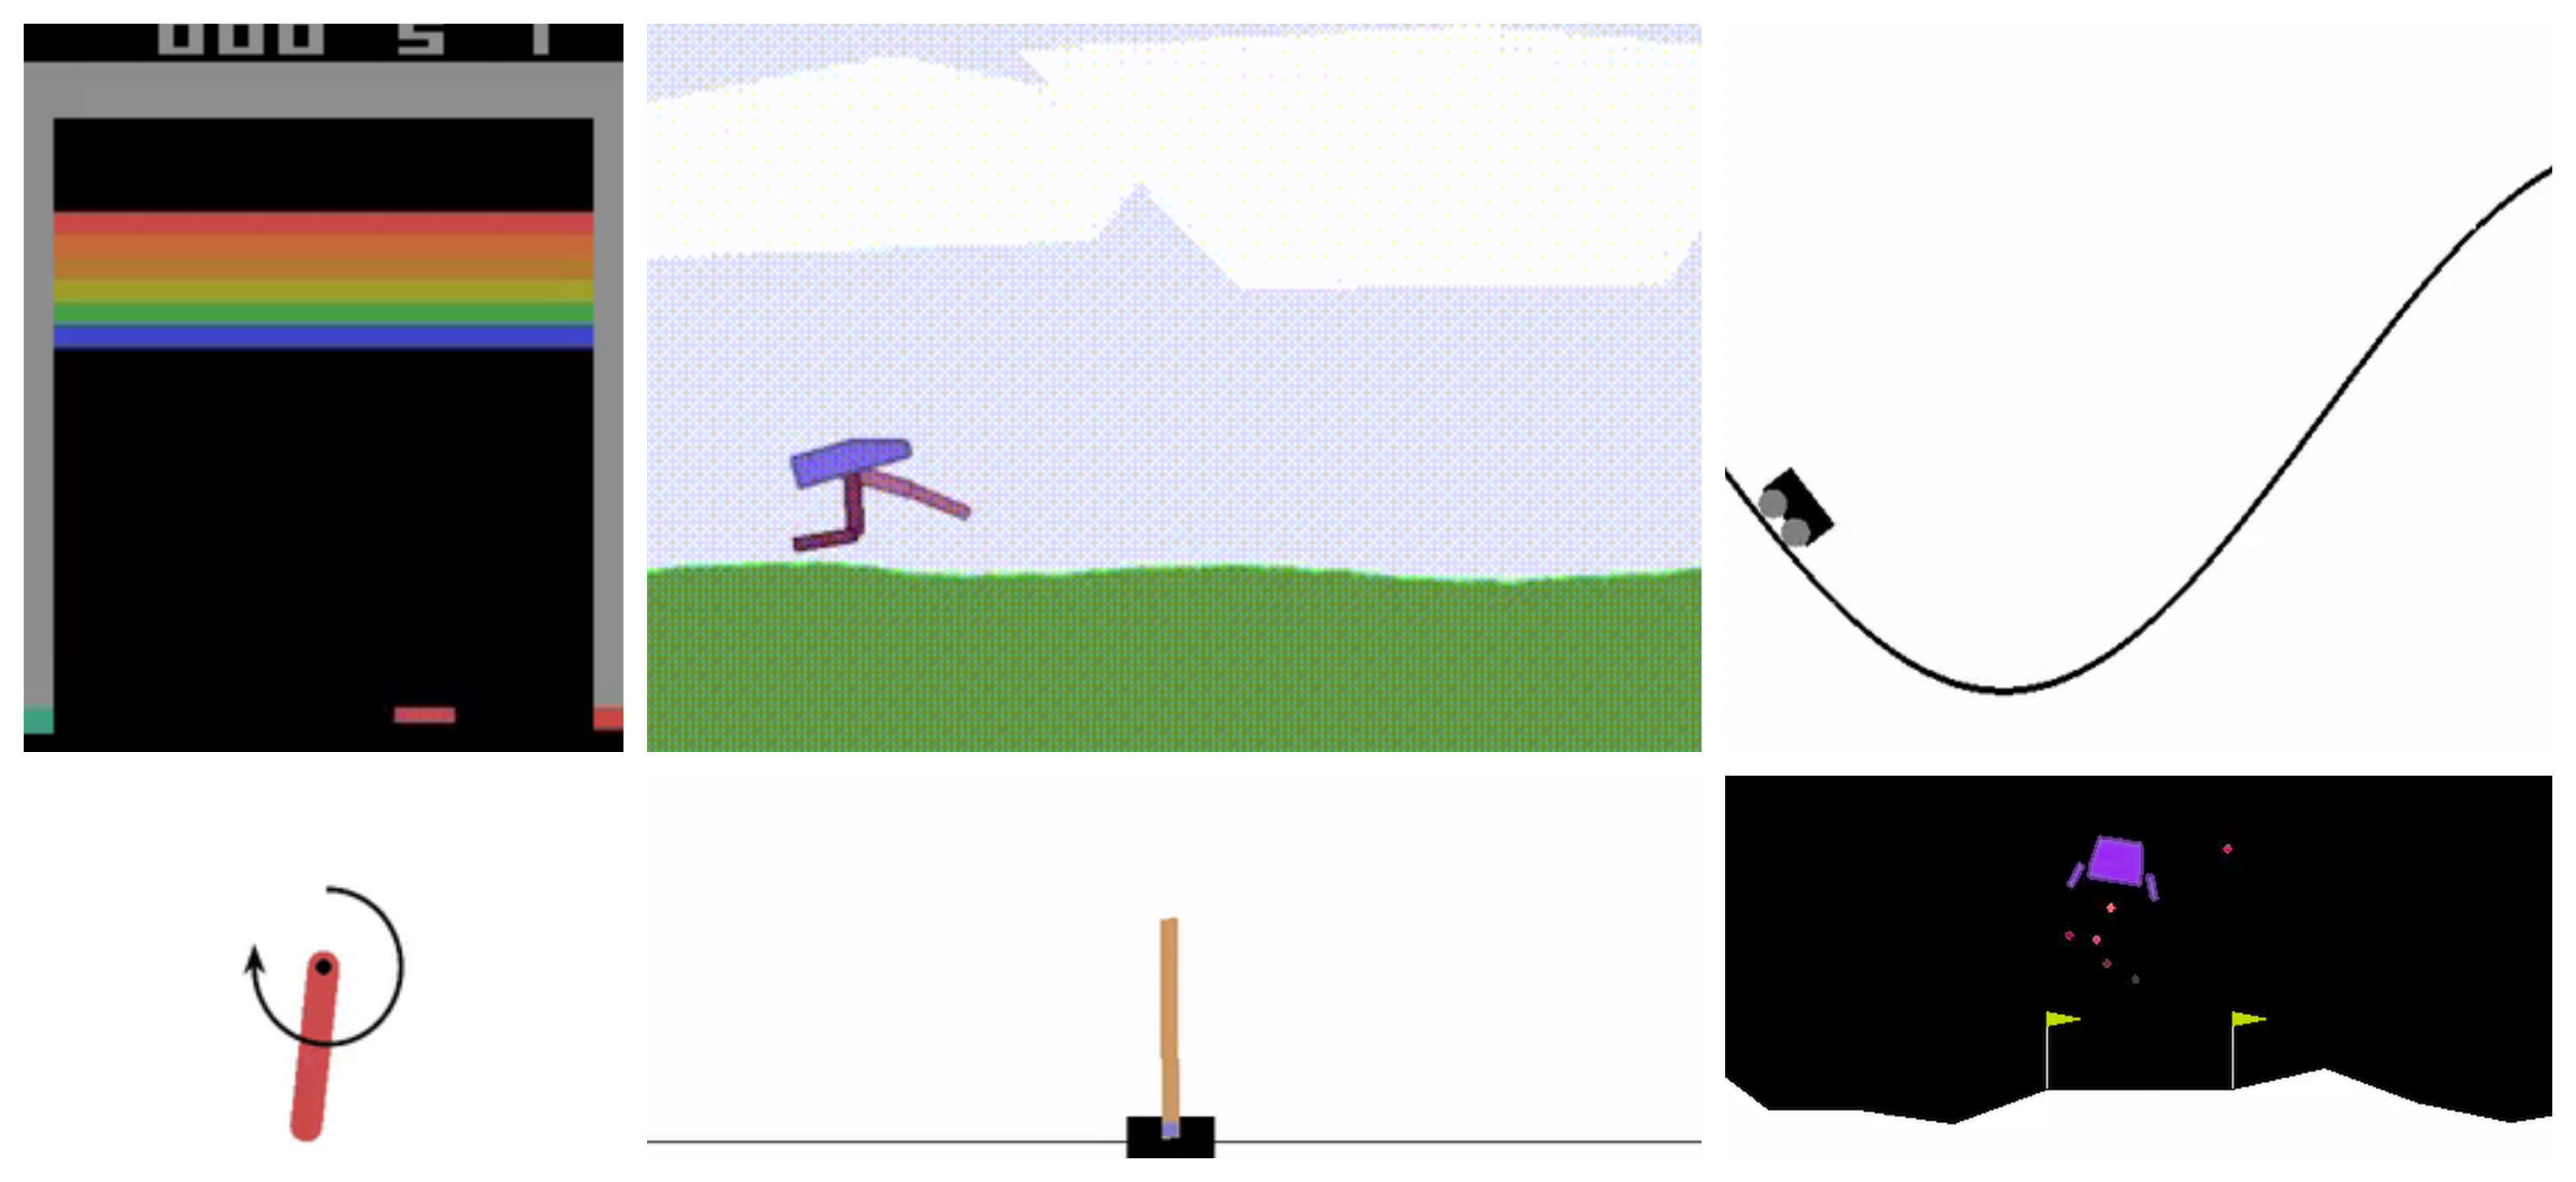
\includegraphics[width=1\columnwidth]{./figures/chapter_3/openaigym.jpg}
    \caption{Diferentes entornos de OpenAI Gym.\label{fig:openai-gym}}
\end{figure}

En este Trabajo Fin de Máster se utiliza la interfaz de OpenAI Gym en su versión $0.16.0$ para construir un entorno similar pero añadiendo la funcionalidad necesaria para acoplar ROS como herramienta de comunicación y Gazebo como herramienta de representación. Esta agregación se materializa en forma de librería, llamada Gym-Gazebo.


%%%%%%%%%%%%%%%%%%%%%%%%%%%%%%%%%%%%%%%%%%%%%%%%%%%%%%%%%%%%%%%%%%%%%%%%%%%%%%%%%%%%%%%%%%%%%%%%%%%%%%%%%%%%%%%%
\section{Gym Gazebo}

El núcleo principal del proyecto donde se desarrolla el código que resuelve el problema planteado se localiza en la librería Gym-Gazebo~\cite{paper_gym_gazebo}, escrita en Python en su versión 2.7. La librería pertenecía a la empresa \textit{Erle Robotics} hasta que fue adquirida por Acutronic\footnote{\url{http://www.acutronic.com/ch/}}. En ese momento, el repositorio\footnote{\url{https://github.com/erlerobot/gym-gazebo}} dejó de tener soporte y fue cerrado para la contribución pero continúa a disposición de la comunidad para ser utilizado como plataforma para el aprendizaje por refuerzo.\\

Gym-Gazebo facilita el desarrollo de algoritmos de aprendizaje por refuerzo aplicados a la robótica usando el mismo interfaz de funciones que utiliza OpenAI Gym y combinándolos con estándares como ROS y Gazebo para las comunicaciones y simulación. Inicialmente parte de varios escenarios donde se utilizan distintos tipos de algoritmos para la resolución como Q-learning o SARSA empleando distintos tipos de sensores como LIDAR o láser combinado con los motores de Gazebo para la resolución de problemas como esquivar obstáculos, navegación, etc. En la figura \ref{fig:mundos-gym-gazebo} pueden verse algunos de estos escenarios.


\begin{figure}
  \begin{center}
    \subfloat[Laberinto.]{\label{fig:laberint}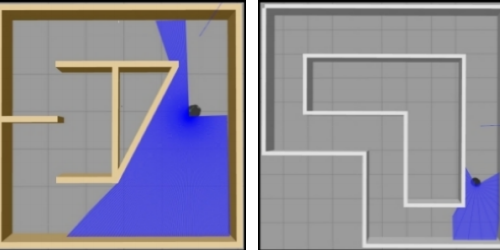
\includegraphics[width=.46\linewidth]{figures/chapter_3/gym-gazebo-1.png}}
    \hspace{0.1cm}
    \subfloat[Laberinto con obstáculos.]{\label{fig:laberinto-obstaculos}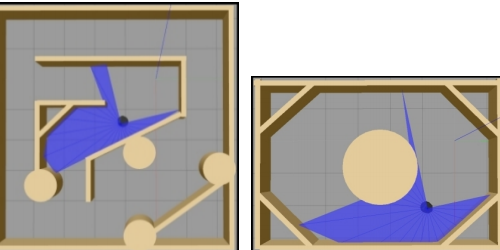
\includegraphics[width=.46\linewidth]{figures/chapter_3/gym-gazebo-2.png}}
  \end{center}
  \centering
  \captionsetup{justification=centering,margin=2cm}
  \caption{Diferentes entornos de Gym Gazebo.}
  \label{fig:mundos-gym-gazebo}
\end{figure}

Los robots disponibles para resolver estos entornos son variados teniendo brazos mecánicos móviles y articulados para ejercicios de coger y soltar y por otro lado también robots \textit{turtlebot}, para la resolución de ejercicios de tipo esquivar obstáculo o avanzar sin colisionar con las paredes, etc. En la figura \ref{fig:robots-gym-gazebo} pueden verse algunos de estos robots.

\begin{figure}
  \begin{center}
    \subfloat[Robot ARIA.]{\label{fig:gym-gazebo-aria}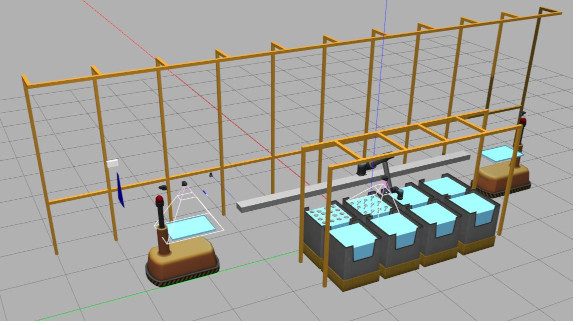
\includegraphics[width=.45\linewidth]{figures/chapter_3/gym-gazebo-aria.jpg}}
    \hspace{0.1cm}
    \subfloat[Brazo articular]{\label{fig:gym-gazebo-brazo}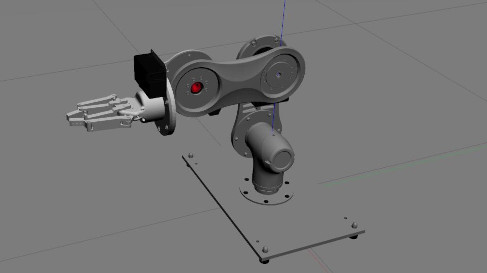
\includegraphics[width=.45\linewidth]{figures/chapter_3/gym-gazebo-brazo-articular.jpg}}
    \hspace{0.1cm}
    \subfloat[Cartpole.]{\label{fig:gym-gazebo-cartpole}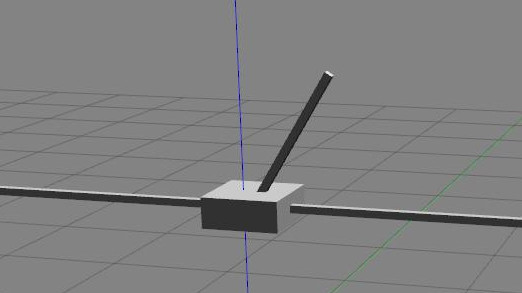
\includegraphics[width=.45\linewidth]{figures/chapter_3/gym-gazebo-cartpole.jpg}}
    \hspace{0.1cm}
    \subfloat[Robot Scara.]{\label{fig:gym-gazebo-scara}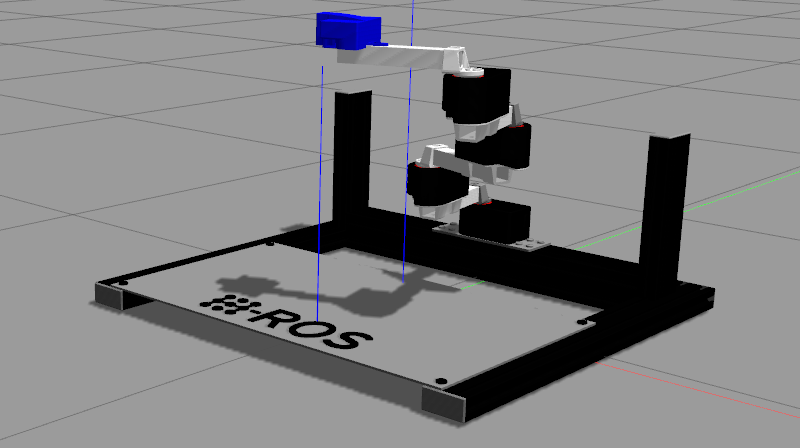
\includegraphics[width=.45\linewidth]{figures/chapter_3/gym-gazebo-scara.png}}
  \end{center}
  \centering
  \captionsetup{justification=centering,margin=2cm}
  \caption{Robots disponibles de Gym-Gazebo.}
  \label{fig:robots-gym-gazebo}
\end{figure}

